	\section{Lower Bounds}\label{sec:lowerbounds}

This section contains three parts.

In~\cref{subsec:warmup}, we will prove that there is no polynomial algorithm solving \oss{n^\epsilon}{1}. The technique is similar to the construction used by Elkin and Peleg~\cite{ElkinP07} to prove the hardness of approximating directed spanner. We will also define \ga{}, as discussed in~\cref{sec:overview}, and prove the hardness for \ga{} when $s=o(m)$.

In~\cref{subsec:bicriterialower}, we will show how to prove the lower bound for \oss{n^\epsilon}{n^\epsilon}, using the lower bound for \ga{} while preserving the relative size of $s$ versus $m$. It will only prove that \oss{n^\epsilon}{n^\epsilon} is hard for some input $s=o(m)$ by combining with the result in~\cref{subsec:warmup}, which is still not what we want in~\cref{thm:main}.

In~\cref{subsec:largebicriteria}, we boost $s$ to be $\omega(m)$ in the lower bound proof of \ga{}. Combined with the lemma proved in~\cref{subsec:bicriterialower}, this will show us \oss{n^\epsilon}{n^\epsilon} is hard for some input $s=\Omega(m^{1+\epsilon})$, which is what we want in~\cref{thm:main}.


\subsection{Warm up: Lower Bounds when \texorpdfstring{$\apxD=1$}{apxD1}}\label{subsec:warmup}

This section will use a simple construction to prove the following lemma.

\begin{lemma}\label{lem:onecriteria}
	Assuming PGC (\cref{con:pgc}), there are no polynomial time algorithm solving \oss{n^{\epsilon}}{1} for some small constant $\epsilon$. 
	
\end{lemma}

The construction relies on the following \minre{} graph.

\begin{definition}[\labcov{} graph]\label{def:minrepgraph}
	Given a \labcov{} instance $\I=(A,B,E,\L,(\pi_e)_{e\in E})$ descirbed in~\cref{def:labcov} and a parameter $\rho$, we define the \labcov{} graph $G_{\I,\rho}$ as a directed graph defined as follows (see \cref{fig:minrepgraph}):
	\begin{itemize}
		\item Suppose $A=\{1,...,|A|\},B=\{1,...,|B|\},\L=\{1,2,...,|\L|\}$. In $G_{\I,\rho}$ we have vertices $\{\aa{i}{j},\bb{i}{j}\mid 1\le i\le |A|=|B|, 1\le j\le |\L|\}$ and edges $\{(\aa{i}{j},\bb{i'}{j'})\mid (i,i')\in E, (j,j')\in\pi_{(i,i')}\}$.
		
		\item In addition, $G_{\I,\rho}$ also contains vertices $\{\a{i},\b{i}\mid 1\le i,j\le |A|=|B|\}$, where $\a{i}$ has a directed path with length $\rho$ to each vertex in $\{\aa{i}{j}\mid 1\le j\le |\L|\}$ denoted by $\alpha^{(i)}_j$, the vertices along the path are $\{\aaa{i}{j}{k}\mid 1\le k\le \rho-1\}$; similarly, $\b{i}$ has a directed path with length $\rho$ from each vertex in $\{\bb{i}{j}\mid 1\le j\le |\L|\}$ denoted by $\beta^{(i)}_j$, the vertices along the path are $\{\bbb{i}{j}{k}\mid 1\le k\le \rho-1\}$. 
		
		\item Finally, we add edges $(\aaa{i}{j}{k},\a{i}),(\b{i},\bbb{i}{j}{k}),(\aa{i}{j},\a{i})$, $(\b{i},\bb{i}{j})$ for any possible $i,j,k$.
	\end{itemize}
	
\end{definition}

\begin{figure}[H]
	\centering
	\includegraphics[scale=1]{figures/minrepgraph.pdf}
	\setcaptionwidth{0.95\textwidth}
	\caption{\small In this example, $|A|=|B|=|\mathcal{L}|=\rho-1=3$. Suppose $A=\{1,2,3\},B=\{1,2,3\},\mathcal{L}=\{1,2,3\}$, then in this example we have $E=\{(2,2)\}$ and $\pi_{(2,2)}=\{(1,2),(2,3),(3,1)\}$, which corresponds to the three edges in the middle. }\label{fig:minrepgraph}	
\end{figure}


\begin{proof}[Proof of~\cref{lem:onecriteria}]
	Given a \labcov{} instance $\I=(A,B,E,\L,(\pi_e)_{e\in E})$, we use $\AB$ to denote the size of $A$ (and also $B$). We now describe how to distinguish between the case. Notice that $N$ is the input size of the \labcov{} instance $\I$.
	\begin{itemize}
		
		\item (Completeness:) There is a labeling that covers every edge. 
		
		\item (Soundness:) Any multilabeling of cost at most $N^{\epsl{}}(|A|+|B|)$ covers at most $N^{-\epsl{}}$ fraction of edges.             
	\end{itemize}
	According to~\cref{lem:pgc}, this violates PGC. 
	
	If $|E|\le 2\AB n^{\epsl}$, then it cannot be the Soundness case, so we assume $|E|>2\AB n^{\epsl}$. 
	
	First, we use polynomial time to compute the \labcov{} graph $G_{\I,\dia{}}$ with $n$ vertices, where $\dia{}$ is polynomial on $N$ and can be arbitrarily large. 
	Then We run the \oss{n^\epsilon}{1} algorithm with input $G_{\I,\dia{}}$ and parameters $s=2\AB,d=\dia{}+1$. We will prove the following two claims, which will lead to the solution to the \labcov{} problem.
	\begin{claim}\label{clai:caseI}
		If the \labcov{} instance is in case (completness), then $G_{\I,\dia{}}$ has a \ssss{2\AB }{\dia{}+1}. Moerover, for any $(i,j)\in E$, $(\a{i},\b{j})$ has distance at most $3$ after adding this \ss{}. 
	\end{claim}
	\begin{proof}
		Suppose the labeling is $\psi$. For any $i\in A$, we include the edge $(\a{i},\aa{i}{\psi(i)})$ in the \ss{}; for any $i\in B$, we include the edge $(\bb{i}{\psi(i)},\b{i})$ in the \ss{}. The \ss{} has size $2\AB $. Since $(i,j)$ is covered by $\psi$, there exists an edge $(\aa{i}{i'},\bb{j}{j'})$ such that $i'=\psi(i),j'=\psi(j)$. In that case, we have the length 3 path $(\a{i},\aa{i}{i'},\bb{j}{j'},\b{j})$ after adding the \ss{}. This proves the second statement of this lemma. Now we verify the distances between reachable pairs are at most $\dia{}+1$ one by one.
		\begin{enumerate}
			\item (start from $\a{i}$) $\a{i}$ can reach any $\aa{i}{j},\aaa{i}{j}{k}$ with distance at most $\dia{}$, $\a{i}$ can reach any $\b{j}$ with $(i,i')\in E$ with distance $3$, which means $\a{i}$ can reach any $\bbb{i'}{j}{k},\bb{i'}{j}$ with distance $4$.
			
			\item (start from $\aaa{i}{j}{k},\aa{i}{j}$) $\aaa{i}{j}{k}$ or $\aa{i}{j}$ has an edge to $\a{i}$, so they can reach any node that $\a{i}$ can reach with distance at most $\dia{}+1$. 
			
			\item (start from $\bbb{i}{j}{k},\bb{i}{j},\b{i}$) These nodes can reach any reachable nodes with distance at most $\dia{}+1$ in $G_{\I,\dia{}}$. 
		\end{enumerate}
		
	\end{proof}
	
	\begin{claim}\label{clai:caseII}
		If the \minre{} instance is in case (soundness), then $G_{\I,\dia{}}$ does not have a \ssss{2\AB\cdot n^{\epsilon}}{\dia{}+1} for sufficiently small constant $\epsilon$. Moreover, by adding any shortcut with size at most $2\AB\cdot n^{\epsilon}$, at most $o(1)$ fraction of pairs in $\{(a^{(i)},b^{(j)})\mid (i,j)\in E\}$ will have distance less than $\dia{}+1$. 
	\end{claim}
	\begin{proof}
		Suppose $G_{\I,\dia{}}$ has a shortcut $E'$ adding which reduces the diameter between $\Omega(1)$ fraction of pairs in $\{(a^{(i)},b^{(j)})\mid (i,j)\in E\}$ to less than $\dia{}+1$. We will try to get a contradiction. We first use $E'$ to build a \mlab{} $\psi$ in the following way: for any $1\le i\le |A|$, we let $\psi(i)$ to be the set of vertices among $\{\aa{i}{j}\mid 1\le j\le \L\}$ that $\a{i}$ has distance at most $\dia{}-1$ to after adding the \ss{}. 
		
		\paragraph{$\psi$ covers more than $N^{-\epsl}$ fraction of edges.}	We first argue that $\psi$ covers $\Omega(1)$ fraction of the edges. Write $A_i=\{\a{i},\aa{i}{j},\aaa{i}{j}{k}\mid 1\le j\le \L,1\le k\le \dia{}-1\}, B_i=\{\b{i},\bb{i}{j},\bbb{i}{j}{k}\mid 1\le j\le \L,1\le k\le \dia{}-1\}$. For an edges $(i,j)\in E$ (recall that $E$ is the edge set in the \labcov{} instance $\I$), we say it is \emph{crossed} if there is an edge $(u,v)\in E'$ with $u\in A_i,v\in B_j$ in $E'$. Remember that we assumed $|E|\ge \Delta\cdot N^{\epsl{}}$, otherwise, the case (soundness) can never happen. Therefore, the number of crossed edges is at most $2\AB\cdot n^{\epsilon}=o(|E|)$ for sufficiently small $\epsilon$. Now We prove that for any non-crossed edge $(i,j)\in E$ such that $(a^{(i)},b^{(j)})$ has distance less than $\dia{}+1$ after adding $E'$, $(i,j)$ is covered by $\psi$. If we can prove this, then at least $\Omega(1)$ fraction of edges in $E$ are covered. To prove this, notice that if $(i,j)$ is not covered, then consider the shortest path $p$ from $\a{i}$ to $\b{j}$ after adding the \ss{}, we write the part where $p$ is inside $A_i$ as $p_A$, and the part where $p$ is inside $B_j$ as $p_B$. if both $p_A,p_B$ has length at most $\dia{}-1$, then $(i,j)$ is covered. Thus, one of $p_A$ or $p_B$ has length at least $\dia{}$. Then we have $|p|=|p_A|+1+|p_B|\ge \dia{}+1+1\ge \dia{}+2$, which is a contradiction. 
		
		\paragraph{$\psi$ has cost at most $N^{\epsl}(|A|+|B|)$.} Then we argue that $\sum_{u\in A\cup B}|\psi(u)|\le |E'|\le 2\AB \cdot n^{\epsilon}$ (which will give us $\sum_{u\in A\cup B}|\psi(u)|\le N^{\epsl{}}(|A|+|B|)$ for sufficiently small $\epsilon$). For a label $j\in\psi(i)$, we have $\distt{(V,E\cup E')}{\a{i},\aa{i}{j}}<\dia{}$. Thus, there exists a path $p=(v_0,...,v_{\ell})$ from $\a{i}$ to $\aa{i}{j}$ with length at most $\dia{}-1$. Let $p'=(\a{i},\aaa{i}{j}{1},\aaa{i}{j}{2},...,\aa{i}{j})$. Let $k$ be the last index such that $v_k\not\in p'$ and $v_{k+1}\in p'$. Since $v_{\ell}$ in $p'$ and the length of $p'$ equals $\dia{}$, such $k$ must exist. Since $(v_k,v_{k+1})\not\in E$, we have $(v_k,v_{k+1})\in E'$. We call this edge $(v_k,v_{k+1})$ a \emph{critical edge} of $(i,j)$. For different $i$ and $j$ with $j\in\psi(i)$, they have different critical edges in $E'$ because the corresponding $v_{k+1}$ is always different. Thus, $\sum_{u\in A\cup B}|\psi(u)|\le |E'|\le 2\AB \cdot n^{\epsilon}$.
		
	\end{proof}
	
	If the \labcov{} instance is in case (completeness), by~\cref{clai:caseI}, $G_{\I,\dia{}}$ admits a \ssss{2\Delta}{\dia{}+1}, which means the output by the \oss{n^{\epsilon}}{1} algorithm will be a \ssss{2\Delta\cdot n^{\epsilon}}{\dia{}+1}; on the other hand, if the \labcov{} instance is in case (soundness), by~\cref{clai:caseII}, the output cannot be a \ssss{2\Delta\cdot n^{\epsilon}}{\dia{}+1} since $G_{\I,\dia{}}$ does not have one. Since checking whether the output is \ssss{2\Delta\cdot n^{\epsilon}}{\dia{}+1} or not is in polynomial time, \labcov{} is solved in polynomial time.
 
\end{proof}






In the following definition, we will abstract all the necessary properties of graph $G_{\I,d}$ in a black box that we are going to use to prove the hardness for \oss{n^{\epsilon}}{n^\epsilon}.

\begin{definition}\label{def:gadget}
	For $1>\epsilon,\cs{}>0$, the \gadget{\cs{}}{\epsilon} problem has inputs
	\begin{enumerate}
		\item a directed connected graph $G=(V,E)$ with $m$ edges, $n$ nodes and diameter polynomial on $m$, let the diameter be $d$,
		\item two sets $L,R\subseteq V$ with $L\cap R=\emptyset$, where $|L|$ is polynomial on $m$,
		\item a set of reachable vertex pairs $P\subseteq L\times R$,
		\item a positive integer $s=\Omega(m^{\cs{}})$.
	\end{enumerate}
	The problem asks to distinguish the following two types of graphs.
	\begin{description}
		\item[Type 1.] There exists a \ss{} $E'$ of $G$ with size $s$ such that all reachable pairs $(u,v)\in L\times R$ have distance $O(1)$ after adding $E'$ to $G$.
		\item[Type 2.] By adding any \ss{} with size $s\cdot n^\epsilon$, at most $o(1)$ fraction of the pairs in $P$ have distance at most $d/3$.
	\end{description}
	
\end{definition}

The following lemma shows that~\cref{fig:minrepgraph} is a hard instance for \gadget{\cs{}}{\epsilon}.
\begin{lemma}\label{lem:smallgadget}
	Under PGC (\cref{con:pgc}), there exist constants $\epsilon,\cs{}$ such that \gadget{\cs{}}{\epsilon} cannot be solved in polynomial time.
	
\end{lemma}
\begin{proof}
	Given any \labcov{} instance $\I=(A,B,E,\L,\pi)$ (we write $|A|=\AB$), we construct a \gadget{\cs{}}{\epsilon} instance with the following inputs.
	\begin{enumerate}
		\item The graph is $G_{\I,\dia{}}$ (see~\cref{def:minrepgraph}) for $\dia{}$ arbitrarily large such that $\dia{}$ is polynomial on $N$ (the bit length of instance $\I$). $G_{\I,d}$ has diameter $d=2\dia{}+1$.
		\item $L=\{a_i\mid 1\le i\le \AB\},R=\{b_i\mid 1\le i\le \AB\}$, clearly $|L|=|R|\le m$ and $|L|$ is polynomial on $m$.
		\item $P=\{(a_i,b_j)\mid (i,j)\in E\}$.
		\item $s=|A|+|B|$, it is polynomial on $m$.
	\end{enumerate}
	
	Now we prove that if we have a polynomial time algorithm to distinguish the two types of graphs as described in~\cref{def:gadget}, then we can solve \labcov{} in polynomial time.
	
	If $\I$ is in case (completeness), according to~\cref{clai:caseI}, by adding a \ss{} with size $s=(|A|+|B|)$, all reachable pairs $(a_i,b_j)$ (with $(i,j)\in E$) has distance at most 3. 
 
 If $\I$ is in case (soundness), according to~\cref{clai:caseII}, by adding a \ss{} with size less than $s\cdot n^{\epsilon}$ for sufficiently small $\epsilon$, at most $o(1)$ fraction of pairs in $P$ has distance less than $(2d+1)/3<\dia{}$. 
\end{proof}

\subsection{Lower Bound when \texorpdfstring{$\apxD>1$}{apxDge1} and \texorpdfstring{$s=o(m)$}{0<cs<1}}\label{subsec:bicriterialower}
In this section, we prove the following lemma, which shows how to use the hardness of \gadget{\cs{}}{\epsilon} to get lower bounds for $\apxD>1$.
\begin{lemma}\label{lem:usegadget}
	For any constant $1>\epsilon,\cs{}>0$, if there is no polynomial algorithm solving \gadget{\cs{}}{\epsilon}, then for sufficiently small constant $\gamma$, there is no polynomial algorithm solving \oss{n^{\gamma\epsilon}}{n^{\gamma\epsilon}} even if the input is restricted to $s=\Omega(m^{1+\gamma(\cs{}-1)})$.
	
\end{lemma}
By combining \cref{lem:smallgadget,lem:usegadget}, we can get the following corollary. Notice that this corollary is not the same as~\cref{thm:main}, since it does not restrict $s$ to be $\omega(m)$.

\begin{corollary}\label{cor:smallmain}
	Under \conj{} (\cref{con:pgc}), there is no polynomial algorithm solving \oss{n^{\epsilon}}{n^{\epsilon}} for sufficiently small constant $\epsilon$.
\end{corollary}

The following geometric graph~\cite{HuangP21} is a crucial part of our proof for~\cref{lem:usegadget}. We say a graph $G=(V,E)$ is a $k$-layered directed graph if $V=V_1\uplus V_2\uplus...\uplus V_k$ ($V$ is partitioned into $V_1,...,V_k$), such that for any edge $(u,v)\in E$, there exists $1\le i<k$ and $u\in V_i,v\in V_{i+1}$. $V_i$ is called the $i$-th layer of $G$.

\begin{lemma}[Section 2.2~\cite{HuangP21}]\label{lem:geograph}
	For any $\AB\in\mathbb{N}^+$, for arbitrary constant $0<\lan{}< 1$, we can compute in polynomial time a $\AB^\lan$ layered graph $G=(V,E)$, a set of pairs $P$ and an indexing $\idx{}$ satisfying the following properties.
 
	\begin{enumerate}
            \item Each layer of $G$ contains $\The{\AB^{10}}$ vertices and has a maximum in-degree and out-degree of at most $\AB$. Let the first layer be denoted as $V_1 = \{s_1, s_2, \dots, s_{K_1}\}$ and the last layer as $V_2 = \{t_1, t_2, \dots, t_{K_2}\}$. \label{geoitem1}

		\item $P \subseteq [K_1] \times [K_2]$. For every $i\in[K_1]$, there are $\Omega(\Delta^2)$ pairs $(i,j)\in P$. For every $(i,j)\in P$, there is a unique path from $s_i$ to $t_j$ in $G$, denoted by $p_{i,j}$. $p_{i,j}$ and $p_{i',j'}$ shares at most one edge for different pairs $(i,j)\not=(i',j')$. \label{geoitem3}
		\item The function $\idx{}$ assigns a value from $[\Delta]$ to each $(v, e)$ pair, where $e$ is either an in-edge or an out-edge of vertex $v$. For a given vertex $v$, $\idx{}$ assigns distinct values to its different in-edges, and similarly, $\idx{}$ assigns distinct values to its different out-edges.  For any $(x,y)\in[\AB]\times[\AB]$, there exists $\Omega(\Delta^{10})$ paths $p_{i,j}$ (where $(i,j)\in P$) such that for any edge $(u,v)$ on $p_{i,j}$,\label{geoitem4}
                \begin{itemize}
                    \item if $v$ is in the even layer, then $\Idx{v,(u,v)}=x$, 
                    \item if $u$ is in the even layer, then $\Idx{u,(u,v)}=y$.
                \end{itemize}
	\end{enumerate}
 
\end{lemma}
\begin{proof}[Proof of~\cref{lem:geograph}]
	The general idea is to use the graph described in Section 2.2~\cite{HuangP21} with max degree $\Delta$, and cut the first $\Delta^{\lan{}}$ layers to get our disired graph. Readers are recommanded to read the construction in Section 2.2~\cite{HuangP21}, and the construction for~\cref{lem:geograph} is followed straightforwardly. 
	
	Let the graph $G_1\otimes G_2$ described in Section 2.2~\cite{HuangP21} with parameters $d_1=d_2=2,r_1=\Delta^{3/2}$ be $G_{\Delta}$. $G_{\Delta}$ has $\Omega(\Delta)$ layers, where each layer has $\The{\Delta^{10}}$ vertices. The max in/out-degree is $\Delta$. We use the subgraph of $G_{\Delta}$ induced by the first $\Delta^{\lan{}}$ layers
	to get the desired graph described in~\cref{lem:geograph}, denoted by $G'_{\Delta}$. %
	We construct $P$ in the following way. According to Section 2.2~\cite{HuangP21}, there exist $\Omega(\Delta^{12})$ \emph{Critical Pairs} in $G_{\Delta}$ between the first and last laryer nodes where each of them has a unique path connecting them. We cut each unique path at the first $\Delta^{\lan{}}$ layers, resulting in $\Omega(\Delta^{12})$ pairs between the first and last layer in $G'_{\Delta}$. %
	Now we verify the properties of $P$ one by one.
	\begin{enumerate}
		\item In Section 2.2~\cite{HuangP21}, each critical pairs is $((a,b,0),(a+Dv,b+Dw,2D))$ for some $v,w\in\mathcal{V}_2(r_1)$. There are $\Delta$ possible choices for $v$ or $w$. Thus, for every $a$, there are $\Omega(\Delta^2)$ choices of $b$ such that $(a,b)\in P$.
		\item If the path between $(a,b)\in P$ is not unique, then the path between two critical pair in $G_{\Delta}$ is also not unique.
		\item Since every two path between two critical pairs in $G_\Delta$ share at most one edge according to Lemma 2.6~\cite{HuangP21}, our path segments in the first $\Delta^{\lan{}}$ layers also share at most one edge.
	\end{enumerate}

        Now we construct $\idx{}$. We fix an order for the set $\mathcal{V}_2(r_1)=\{w_1,w_2,...,w_\Delta\}$. Each node in the even layer $(a,b,i)$ has out-edges $\{(a+w_j,b,i+1)\left((a,b,i),(a+w_j,b,i+1)\right)\mid j\in[\Delta]\}$. $\idx{}$ assign index $j$ to the edge $\left((a,b,i),(a+w_j,b,i+1)\right)$. $(a,b,i)$ has in-edges $\{\left((a,b-w_j,i-1),(a,b,i)\right)\mid j\in[\Delta],b-w_j\in B_2(R_1+\left\lceil (i-1)/2\right\rceil r_1)\}$. $\idx{}$ assign $j$ to the edge $\left((a,b-w_j,i-1),(a,b,i)\right)$. Now for any $(x,y)\in[\Delta]\times[\Delta]$, we consider all the unique paths from $(a,b,0)$ to $(a+\Delta^{\lan{}}x,b+\Delta^{\lan{}}y,\Delta^{\lan{}}-1)$. All edges in this path is either $\left((a+ix,b+iy,2i),(a+(i+1)x,b+iy,2i+1)\right)$, which is the in-edge of $(a+(i+1)x,b+iy,2i+1)$ assigned as $x$, or $((a+(i+1)x,b+iy,2i+1)$,$(a+(i+1)x,b+(i+1)y,2i+2))$, which is the out-edge of $(a+(i+1)x,b+iy,2i+1)$ assigned as $y$.\footnote{To avoid confusion, notice that in Section 2.2~\cite{HuangP21}, the node $(x,y,i)$ is in the $(i+1)$-th layer, because $i$ is indexed from $0$. }
\end{proof}
Now we are ready to prove the main lemma in this section.
\begin{proof}[Proof of~\cref{lem:usegadget}]
	Suppose $\mathcal{A}$ is the polynomial time algorithm for \oss{n^{\gamma\epsilon}}{n^{\gamma\epsilon}} where input must satisfy $s=\Omega(m^{1+\gamma(\cs{}-1)})$. Given a \gadget{\cs{}}{\epsilon} instance $G_{inr},(L,R),P',\bufs$ (see~\cref{def:gadget}, we use $G_{inr},P',s'$ instead of $P,s$ to avoid conflicting of notations), we will show how to use $\mathcal{A}$ as an oracle to solve it in polynomial time.
	
	\paragraph{Definition of $G$.} Let $\Delta=|L|=|R|$, let $M$ denote the number of edges in $G_{inr}$ and let the diameter of $G_{inr}$ be $\rho{}$. We first construct a graph $G$ in the following way. Let the graph, pairs, and indexing described in~\cref{lem:geograph} with parameter $\AB$ and sufficiently small constant $\lan$ be $G_{geo},P,I$. Without loss of generality, we assume $\AB^\lan$ is odd. 
	$G$ contains the following parts. See~\cref{fig:origin} as an example.
	
	\begin{figure}
		\centering
		\includegraphics[scale=0.8]{figures/origin.pdf}
		\setcaptionwidth{0.95\textwidth}
		\caption{Suppose the graph above is the graph $G_{geo}$ with $\AB=2$ (notice that for ease of explanation, the graph does not satisfy properties described in~\cref{lem:geograph}). The graph below shows how we substitute each node $v$ by $G_v$. If $v$ is in the even layer, then $G_v$ is a copy of $G_{inr}$; otherwise, if $v$ is not in the first or last layer, $G_v$ is a star graph. }\label{fig:origin}	
	\end{figure}
	
	\begin{enumerate}
		\item (Substitute nodes in even layers by copies of $G_{geo}$) for each vertex $v$ in the even layers of $G_{geo}$, create a copy of graph $G_{inr}$, denoted as $G_v$ as part of $G$. Suppose $L=\{a_1,...,a_{\Delta}\},R=\{b_1,...,b_\Delta\}$ (remember that $L,R$ are inputs to \gadget{\cs{}}{\epsilon}). $a_i$ and $b_i$ are denoted by $a^v_i,b^v_i$ in $G_v$. 
		\item (Substitute nodes in odd layers by star graphs) for each vertex $v$ in the odd layers except the first and last layer of $G_{geo}$, create vertices $s_1,...,s_{\Delta},t_1,...,t_\Delta,v$, and create edges $(s_1,v),,...,(s_\Delta,v),(v,t_1),...,(v,t_\Delta)$.
		\item (Keep first and last layer) remember that $I$ is the input to \gadget{\cs{}}{\epsilon}. $G$ includes all nodes in the first and last layer of $G_{geo}$, denoted by $s_1,s_2,...,s_{K_1}$ and $t_1,t_2,...,t_{K_2}$.
		\item (Edges connected different parts) for each edge $e=(u,v)$ in $G_{geo}$, create an edge $(b^u_{\Idx{u,e}},a^v_{\Idx{v,e}})$ in $G$. If $u$ is in the first layer or $v$ is in the last layer, just create edge $(u,a^v_{\Idx{v,e}})$ or $(b^u_{\Idx{u,e}},v)$ instead.
	\end{enumerate}
	
	Remember that $G_{geo}$ has $\Delta^{\lan{}}$ layers, each with $\Delta^{10}$ vertices, and the max degree of $G_{geo}$ is $\Delta$. The number of edges $m$ in $G$ can be calculated as
	\[m=\The{\Delta^{10+\lan{}}\cdot M}+\The{\Delta^{10+\lan{}}\cdot \Delta}+O(\Delta^{10+\lan{}}\cdot \Delta)=\The{\Delta^{10+\lan{}}\cdot(\Delta+M)}\]
	
	\paragraph{Use $\mathcal{A}$ to solve \gadget{\cs{}}{\epsilon}.} After constructing $G$, we apply $\mathcal{A}$ on $G$ with parameter $s=\AB^{10+\lan}\cdot \bufs, d=C\rho$ for sufficiently large constant $C$. We first argue that $s=\Omega(m^{1+\gamma(\cs{}-1)})$ for sufficiently small $\gamma$ so this is a valid input. Remember that $\bufs$ is one of the inputs to \gadget{\cs{}}{\epsilon} such that $s'=\Omega(M^{\cs{}})$. Also remember in~\cref{def:gadget}, we require $|L|=|R|=\Delta\le M$ to be polynomial on $M$. Denote $M=\Delta^{c_{\Delta}}$. Then we have $m=\The{\Delta^{10+\lan{}+c_\Delta}}$ and $s=\Delta^{10+\lan{}+c_{\Delta}\cs{}}$. Now we have $s/m=\The{\Delta^{c_\Delta(\cs{}-1)}}$, where $\Delta^{c_\Delta}=m^{\gamma}$ for some constant $\gamma$. Thus, we have $s=\Omega(m^{1+\gamma(\cs{}-1)})$.
	
Remember that $\rho$ is the diameter of $G_{inr}$. According to~\cref{def:gadget}, $\rho{}$ is polynomial on $M$. Let $\rho{}= M^{c_D}$. %
Remember our goal is to distinguish the following two types of \gadget{\cs{}}{\epsilon} instances.

\begin{description}
	\item[Type 1.] There exists a \ss{} $E'$ of $G_{inr}$ with size $O(s')$ such that all reachable pairs $(u,v)\in L\times R$ have distance $O(1)$ after adding $E'$ to $G_{inr}$.
	\item[Type 2.] By adding any \ss{} with size $\bufs\cdot M^{\epsilon}$, at most $o(1)$ fraction of the pairs in $P'$ have distance at most $\rho{}/3$.
\end{description}

We prove the following two lemmas to show the output of $\mathcal{A}$ suffices to distinguish whether the \gadget{\cs{}}{\epsilon} instance is in type 1 or type 2. %

\begin{lemma}\label{lem:type1}
	If the \gadget{\cs{}}{\epsilon} instance is type 1, then $G$ has a \ssss{s=\AB^{10+\lan}\cdot \bufs}{O(\rho{})}.
\end{lemma}
\begin{proof}
	For each copy of $G_{inr}$ (denoted as $G_v$) in $G$, we add $\bufs$ edges to the \ss{} to make all reachable pairs $(a^v_{i},b^v_j)$ have distance $O(1)$. The \ss{} has size at most $\AB^{10+\lan}\cdot \bufs$. Consider a reachable $(u,v)$ in $G$, we first argue that they have distance $O(\rho{}+\AB^\lan)$ after adding the \ss{}. To see this, notice that a path connecting $u,v$ can only be in the form of $(u,p_1,p_2,...,p_{\ell},v)$ where $p_i$ is a path inside $G_v$ for some $v$, and $\ell\le\AB^{\lan}$. %
	Each $p_i$ with $1<i<\ell$ will be in the form $(a^v_i,...,b^v_j)$ for some $v,i,j$. Notice that $(a^v_i,b^v_j)$ has distance $O(1)$ after adding the shortcut if $v$ is in the even layer (if $v$ is in the odd layer then there is already an existing length 2 paths connecting $(a^v_i,b^v_j)$). Therefore, $u$ has distance $O(\rho{}+\AB^\lan)$ to $v$. Remember that $\rho{}=M^{c_D}=\Delta^{c_\Delta c_D}$. By setting $\lan{}<c_\Delta c_D$, the distance is at most $O(\rho{})$.
\end{proof}


\begin{lemma}\label{lem:type2}
	If the \gadget{\cs{}}{\epsilon} instance is type 2, then $G$ has no \ssss{n^{\gamma\epsilon}s}{n^{\gamma\epsilon}\rho{}}.
\end{lemma}
\begin{proof}
	
	Before we prove our lemma, we need to do some preparations. %
	Remember that $P'$ is the input to \gadget{\cs{}}{\epsilon} such that for any $(x,y)\in P'\subseteq[\AB]\times[\AB]$, $a^v_x$ can reach $b^v_y$ for any $v$. Also recall that according to~\cref{lem:geograph} item~\ref{geoitem4}, for every $(x,y)\in P'\subseteq [\AB]\times[\AB]$, in $G_{geo}$ there exists $\Omega(\Delta^{10})$ paths $p_{i,j}$ (which is the unique path connecting $s_i,t_j$) that all edges $(u,v)$ in this path is the in-edge indexed by $I$ as $x$ of $v$ if $v$ is in the even layer, or the out-edge indexed by $I$ as $y$ of $u$ if $u$ is in the even layer. That means in $G$, there is a path from $s_i$ to $t_j$ in the form of $p'_{i,j}=(s_i,a^{v_{2,q_2}}_{x},...,b^{v_{2,q_2}}_{y}, a^{v_{3,q_3}}_x,...,b^{v_{3,q_3}}_y,...,t_j)$. We say $p'_{i,j}$ covers vertices $v_{2,q_2},v_{3,q_3},...$ at $(x,y)$. Moreover, for $(i',j')\not=(i,j)$, we know from~\cref{lem:geograph} item~\ref{geoitem3} that $p_{i,j},p_{i',j'}$ shares at most one edge. Thus, $p'_{i,j}$ and $p'_{i',j'}$ cannot cover the same vertex $v$ at the same $(x,y)$, otherwise they share two edges: the in-edge indexed as $x$ of $v$ and the out-edge indexed as $y$ of $v$. In summary, we have $\Omega(\Delta^{10}|P'|)$ pairs $(i,j)$, which we call critical pairs, satisfying the following properties.
	\begin{enumerate}
		\item $s_i$ can reach $t_i$ in $G$, where all paths from $s_i$ to $t_i$ must be in the form $(s_i,a^{v_{2,q_2}}_{x},...,b^{v_{2,q_2}}_{y}, a^{v_{3,q_3}}_x,$ $...,b^{v_{3,q_3}}_y,...,t_j)$. 
		\item Any path from $s_i$ to $t_j$ cover one vertex $v$ in each layer at some pair $(x,y)\subseteq P'$. For different critical pairs $(i,j)\not=(i',j')$, they will not cover the same vertex $v$ at the same pair $(x,y)\subseteq P'$.
	\end{enumerate} 
	
	
	Now we are ready to prove \cref{lem:type2}. We will prove that $G$ does not have a \ssss{\AB^{10+\lan}\cdot \bufs\cdot M^{\epsilon/2}}{\rho{}\AB^{\lan}/9}. We first show why this implies~\cref{lem:type2}. Remember that $s=\AB^{10+\lan}\cdot \bufs$, thus, $\AB^{10+\lan}\cdot \bufs\cdot M^{\epsilon/2}>m^{\gamma\epsilon}s)$ for sufficiently small constant $\gamma$. Also remember that $m$ is polynomial on $\Delta$, thus, $\rho{}\Delta^{\lan{}}/9>m^{\gamma\epsilon}\rho{}$ for sufficiently small constant $\gamma$. 
	
	Suppose to the contrary, $G$ has a \ssss{\AB^{10+\lan}\cdot \bufs\cdot M^{\epsilon/2}}{\rho{}\AB^{\lan}/9}, we will make a contradiction. We first claim that $G$ also has a \ssss{\AB^{10+\lan}\cdot \bufs\cdot M^{\epsilon/2}\cdot \AB^{\lan}}{\rho{}\AB^{\lan}/8}, denoted by $E'$, such that both end points for every edge in $E'$ is in the same layer. We can achieve this by taking any edge $(u,v)$ in the original \ss{} that crosses different layers, finding the path from $u$ to $v$ denoted by $p$, and cut $p$ into at most $\AB^\lan$ segments $p_1,p_2,...,p_\ell$ where each segment is in the same layer, and replace $(u,v)\in E'$ by $\Delta^{\lan}$ new edges each connecting two end points of $p_i$ from $i=1$ to $i=\ell$. In this way, the \ss{} increase by a factor of at most $\AB^\lan$. The distance between two vertices increases by at most an additive factor of $O(\AB^\lan)$. Another property of $E'$ is that every edge in $E'$ has both endpoints in $G_v$ for some $v$. That is because different $G_v$ where $v$ in the same layer are not reachable from each other. 
	
	Now with $E'$ added to $G$, we denote the new graph by $G'$. We define an indicator variable $I_{v,i,j}$ to be $1$ if $\distt{G'}{a^v_i,b^v_j}\le \rho{}/3$. We know from the property of type 2 that for any $v$ and arbitrary small constant $\eta$, $\sum_{i,j\in P'}I_{v,i,j}>\eta|P'|$ implies $E'$ has at least $\bufs\cdot M^{\epsilon}$ edges in $G_v$. Since $|E'|\le \AB^{10+\lan}\cdot \bufs\cdot M^{\epsilon/2}\cdot \AB^{\lan}$, by setting $\lan<1/2$, at most $o(\AB^{10+\lan})$ vertices $v$ has the property that $\sum_{i,j\in P'}I_{v,i,j}>\eta|P'|$, which means $\sum_{v,(i,j)\in P'}I_{v,i,j}\le 2\eta\AB^{10+\lan}|P'|$. However, for each critical pair $(i,j)$, suppose $T_{i,j}=\{(v,x,y)\mid (i,j)\text{ covers }v\text{ at }(x,y)\}$, then we have $\sum_{(v,x,y)\in T_{i,j}}I_{v,x,y}\ge (1/2)\AB^\lan$, otherwise the distance $\distt{G'}{s_i,t_j}$ with be at least $(\AB^\lan)/2\cdot \rho{}/3>\rho{}\AB^\lan/6$. We also know that $T_{i,j}$ is disjoint for different $i,j$. Thus, we get $\sum_{v,i,j}I_{v,i,j}=\Omega(\Delta^{10}|P'|)\cdot \AB^\lan/2=\Omega(|P'|\AB^{10+\lan})$, contradicts the fact that $\sum_{v,i,j}I_{v,i,j}\le 2\eta\AB^{10+\lan}|P'|$ for sufficiently small constant $\eta$. 
	\yonggang{I think this proof is very hard to parse and I should try to refine it.}
	
\end{proof}

If the \gadget{\cs{}}{\epsilon} instance is type 1, then according to~\cref{lem:type1}, $G$ admits a \ssss{s=\AB^{10+\lan}\cdot \bufs}{O(\rho{})}, so $\mathcal{A}$ will output a \ssss{n^{\gamma\epsilon}s}{n^{\gamma\epsilon}\rho{}}; on the other hand, if the \gadget{\cs{}}{\epsilon} instance is type 2, then according to~\cref{lem:type1}, $G$ cannot output a \ssss{n^{\gamma\epsilon}s}{n^{\gamma\epsilon}\rho{}}. Since checking whether an edge set is a \ssss{n^{\gamma\epsilon}s}{n^{\gamma\epsilon}\rho{}} or not is in polynomial time, the output of $\mathcal{A}$ distinguish type 1 from type 2.

\end{proof}

\subsection{Lower Bound when \texorpdfstring{$\apxD>1$}{paxDge1} and \texorpdfstring{$s=\omega(m)$}{cs>1}}\label{subsec:largebicriteria}

In this section, we prove the following lemma.

\begin{lemma}\label{lem:larges}
	Assuming \conj{} (\cref{con:pgc}), there exists two constants $0<\delta,\epsilon<1$ such that \gadget{1+\delta}{\epsilon} cannot be solved in polynomial time.
\end{lemma}
by combining~\cref{lem:larges,lem:usegadget}, we can get the proof of~\cref{thm:main}.
\begin{proof}[Proof of~\cref{thm:main}]
	According to~\cref{lem:larges}, under \conj{}, there exists two constants $0<\delta,\epsilon<1$ such that \gadget{1+\delta}{\epsilon} cannot be solved in polynomial time. According to~\cref{lem:usegadget}, there are no polynomial algorithm solving \oss{m^{\gamma\epsilon}}{m^{\gamma\epsilon}} when input $s=\Omega(m^{1+\gamma(1+\delta-1)})=\Omega(m^{1+\gamma\delta})$ for some constant $\gamma$. 
\end{proof}

\begin{proof}[Proof of~\cref{lem:larges}]
	Given a \labcov{} instance $\I=(A,B,E,\L,(\pi_e)_{e\in E})$ described in~\cref{def:labcov}, \conj{} implies we cannot distinguish the following two cases in polynomial time for some small constant $\epsl{}$ according to to~\cref{lem:pgc}. Remember that $N$ is the input bit length of $\I$.
	
	\begin{itemize}
		\item (Completeness:) There is a labeling that covers every edge. 
		
		\item (Soundness:) Any multilabeling of cost at most $N^{\epsl{}}(|A|+|B|)$ covers at most $N^{-\epsl{}}$ fraction of edges.      	
	\end{itemize}
	
	
	Assuming there is a polynomial time algorithm $\mathcal{A}$ solving \gadget{1+\delta}{\epsilon} for sufficiently small constant $\epsilon$, we will show how to distinguish the above two cases in polynomial time, which will lead to a contradiction.
	
	
	\paragraph{Definition of $G$.} First, we construct a graph $G$ (see~\cref{fig:large}) according to the instance $\I$. Let $\Delta=N^{c_{\Delta}}$ for a sufficiently large constant $c_{\Delta}$. Denote the graph described by~\cref{lem:geograph} with parameter $\Delta$ as $G_{geo}$. Remember that $G_{geo}$ has $\Delta^{\lan{}}$ layers, each with size $\Theta(\Delta^{10})$, where the first layer is $S=\{s_1,s_2,...,s_{K_1}\}$, the last layer is $T=\{t_1,t_2,...,t_{K_2}\}$.
	\begin{enumerate}
		\item $G$ has two sides: $A$ side and $B$ side. Each side contains $K_1$ \emph{batches}, each batch is composed by $|A|=|B|$ \emph{fans}. Let the reversed graph of $G_{geo}$ (where we reverse all the edge directions in this graph) as $G^R_{geo}$. On the $A$ side, each fan is composed of $\L$ copies of graph $G^R_{geo}$; on the $B$ side, each is composed of $\L$ copies of a graph $G_{geo}$. All $G^R_{geo}$ or $G_{geo}$ in the same fan share the same $T$ vertex set. On the $A/B$ side, the $k$-th copied graph in the $i$-th batch, $j$-th fan is denoted by $G^{A/B}_{i,j,k}$, where the node $s_\ell$ in $G_{geo}$ is denoted by $s^{A/B}_{(i,j),\ell}$ for $1\le \ell\le K_1$ (recall that for different $k$, they share the same $s_\ell$), and the node $t_\ell$ in $G_{geo}$ is denoted by $t^{A/B}_{(i,j,k),\ell}$ for $1\le \ell\le K_2$. 
		\item $G$ has edges defined by the \labcov{} instance $\I$ from $A$ side to $B$ side described as follows. Remember that $\I=(A,B,E,\L,(\pi_e)_{e\in E})$ where $A=\{1,2,...,|A|\},B=\{1,2,...,|B|\},\L=\{1,2,...,|\L|\}$. For every $(j,j')\in E,(k,k')\in\pi_{(j,j')}$ and $i,\ell\in[K_1]$, there is an edge from $s^A_{(i,j,k),\ell}$ to $s^B_{(\ell,j',k'),i}$. 
		An intuition of why the edges are defined in this way is that, now if a path is from the $A$ side of the $i$-th batch to $B$ side of the $\ell$-th batch, the path must go through $s^A_{(i,j,k),\ell}$ to $s^B_{(\ell,j',k'),i}$ for some $(j,j')\in E,(k,k')\in\pi_{(j,j')}$.
		\item For every $\ell\in[K_2]$, create a node $p^A_\ell$ and edges $\{(t^A_{(i,j),\ell},p^A_\ell)\mid 1\le i\le K_1,1\le j\le |A|)\}$. For every $i\in[K_1]$, create a node $q^B_i$ and edges $\{(q^B_i,t^B_{(i,j),\ell})\mid 1\le j\le |A|,1\le \ell\le K_2\}$. Remember that in~\cref{lem:geograph}, $P$ is a set of pairs between first and last layer indexes of nodes in $G_{geo}$. For every $\ell\in[K_2],i\in[K_1]$ where $(i,\ell)\not\in P$, we create an edge $(p^A_{\ell},q^B_{i})$. 
		
		We also create a mirror of the above nodes and edges (\cref{fig:large} does not draw) by reversing $A$ and $B$. i.e., for every $\ell\in[K_2]$, create a node $p^B_\ell$ with edges $\{(p^B_\ell,t^B_{(i,j),\ell})\mid 1\le i\le K_1,1\le j\le |A|)\}$. For every $i\in[K_1]$, create a node $q^A_i$ with edges $\{(t^A_{(i,j),\ell},q^A_i)\mid 1\le j\le |A|,1\le \ell\le K_2\}$. For every $\ell\in[K_2],i\in[K_1]$ where $(i,\ell)\not\in P$, we create an edge $(q^A_{i},p^B_{\ell})$. 
	\end{enumerate} 
	
	Remember that the number of edges in $G_{geo}$ is $M=O(\Delta^{11+\lan{}})$. Let $n$ be the number of nodes in $G$. Let $m$ be the number of edges in $G$. $m$ can be calculated as
	\[m={\color{gray}M\cdot K_1|A||\L|}+{\color{blue}O(|\L|^2|A|^2)\cdot K_1^2}+{\color{orange}4K_1K_2|A|}+{\color{red}O(K_1K_2)}=\Theta(M\cdot K_1|A||\L|)\]
	The third and fourth terms are trivially less than the first term. The second term is less than the first term since we set $\Delta=N^{c_\Delta}$ for sufficiently large constant $c_\Delta$. 
	\begin{figure}
		
		\begin{center}
			
			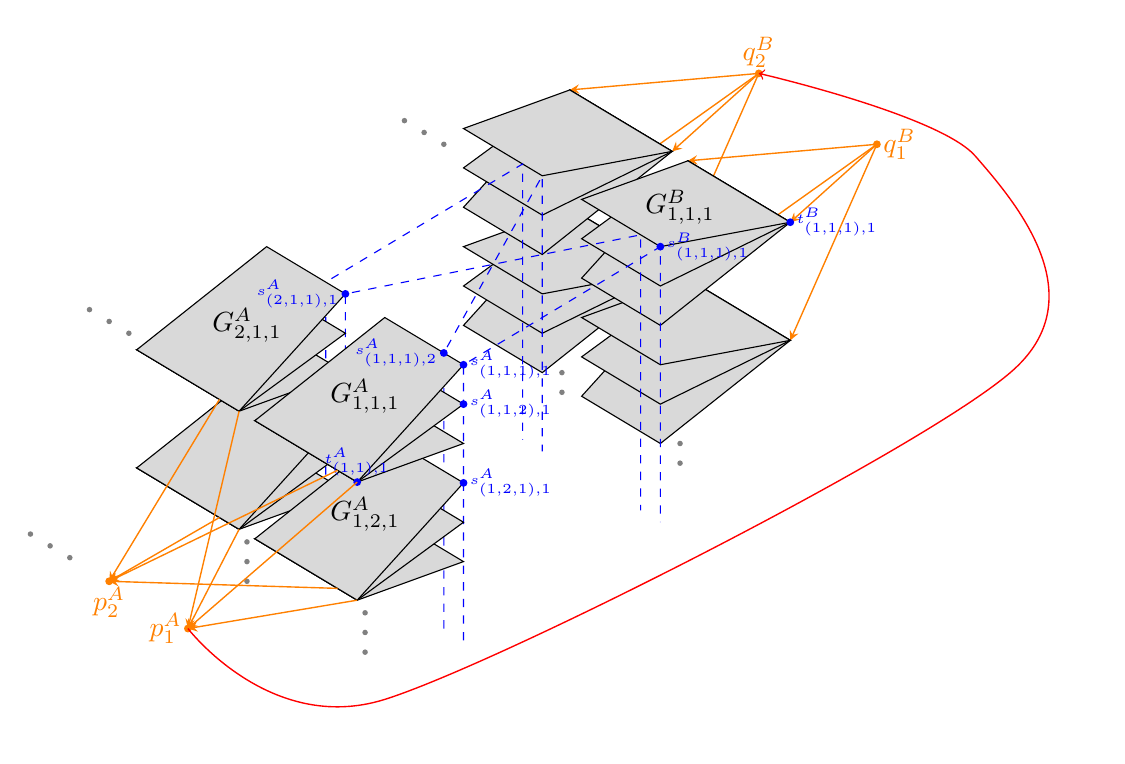
\begin{tikzpicture}[x={(0.5cm,0.3cm)}, y={(-0.5cm,0.3cm)}, z={(0cm,0.5cm)}]
				
				\newcommand{\con}{3}
				
				\newcommand{\drawpiece}[4]{
					\coordinate (A) at (0 * #1 + #2, -0.3 + #3, 0 + #4);
					\coordinate (B) at (0 * #1 + #2, 2.3 + #3, 0 + #4);
					\coordinate (A1) at (3 * #1 + #2, 2 + #3, 1 + #4);
					\coordinate (B1) at (3 * #1 + #2, 0 + #3, 1 + #4);
					\coordinate (A2) at (3 * #1 + #2, 2 + #3, 0 + #4);
					\coordinate (B2) at (3 * #1 + #2, 0 + #3, 0 + #4);
					\coordinate (A3) at (3 * #1 + #2, 2 + #3, -1 + #4);
					\coordinate (B3) at (3 * #1 + #2, 0 + #3, -1 + #4);
					\draw[fill=gray!30] (A) -- (B) -- (A3) -- (B3) -- cycle;
					\draw[fill=gray!30] (A) -- (B) -- (A2) -- (B2) -- cycle;
					\draw[fill=gray!30] (A) -- (B) -- (A1) -- (B1) -- cycle;
					
				}
				\newcommand{\drawstack}[5]{
					\fill[gray] (1.5 * #1 + #2,1 + #3,-2 + #5  + #4) circle (1pt);
					\fill[gray] (1.5 * #1 + #2,1 + #3,-2.5 + #5  + #4) circle (1pt);
					\fill[gray] (1.5 * #1 + #2,1 + #3,-3 + #5  + #4) circle (1pt);
					\drawpiece{#1}{#2}{#3}{#4 + #5}
					\drawpiece{#1}{#2}{#3}{#4}
				}
				\newcommand{\drawbatch}[6]{
					\fill[gray] (1.5 * #1 + #2,7 + #3,-1.5) circle (1pt);
					\fill[gray] (1.5 * #1 + #2,7.5 + #3,-1.5) circle (1pt);
					\fill[gray] (1.5 * #1 + #2,8 + #3,-1.5) circle (1pt);
					\drawstack{#1}{#2}{#3 + #6}{#4}{#5}
					\drawstack{#1}{#2}{#3}{#4}{#5}
				}
				
				\coordinate (qB1) at (15, 1.5,-1.5);
				
				\draw  (qB1) node[circle, fill, inner sep=1pt, label={[label distance=-0.1cm, color = orange]right:\fontsize{10}{0}\selectfont$q^B_{1}$},  color=orange] {};
				
				
				\draw[->, >=stealth, color=orange, line width=0.5pt] (qB1) -- (11,-0.3,0);
				\draw[->, >=stealth, color=orange, line width=0.5pt] (qB1) -- (11,2.3,0);
				
				\draw[->, >=stealth, color=orange, line width=0.5pt] (qB1) -- (11,-0.3,-3);
				\draw[->, >=stealth, color=orange, line width=0.5pt] (qB1) -- (11,2.3,-3);
				\coordinate (qB1) at (15, 1.5,-1.5);
				
				\coordinate (qB2) at (15, 1.5 + 3,-1.5);
				\draw  (qB2) node[circle, fill, inner sep=1pt, label={[label distance=-0.1cm, color = orange]above:\fontsize{10}{0}\selectfont$q^B_{2}$},  color=orange] {};
				
				
				\draw[->, >=stealth, color=orange, line width=0.5pt] (qB2) -- (11,-0.3 + 3,0);
				\draw[->, >=stealth, color=orange, line width=0.5pt] (qB2) -- (11,2.3 +  3,0);
				
				\draw[->, >=stealth, color=orange, line width=0.5pt] (qB2) -- (11,-0.3 +  3,-3);
				\draw[->, >=stealth, color=orange, line width=0.5pt] (qB2) -- (11,2.3 +  3,-3);
				
				\drawbatch{-1}{11}{0}{0}{-3}{3}
				
				\draw[blue, dashed, dash pattern=on 3pt off 3pt] (3,0,-6) -- (3,0,1) -- (5 + \con,0,1) -- (5 + \con,0,-6);
				\draw[blue, dashed, dash pattern=on 3pt off 3pt] (3,0.5,-6) -- (3,0.5,1) -- (5 + \con,3,1) -- (5 + \con,3,-6);
				\draw[blue, dashed, dash pattern=on 3pt off 3pt] (3,3,-6) -- (3,3,1) -- (5 + \con,0.5,1) -- (5 + \con,0.5,-6);
				\draw[blue, dashed, dash pattern=on 3pt off 3pt] (3,3.5,-6) -- (3,3.5,1) -- (5 + \con,3.5,1) -- (5 + \con,3.5,-6);
				
				\drawbatch{1}{0}{0}{0}{-3}{3}
				
				\node at (1.5, 1, 0.5) {$G^A_{1,1,1}$};
				
				\node at (1.5, 4, 0.5) {$G^A_{2,1,1}$};
				
				\node at (1.5, 1, -2.5) {$G^A_{1,2,1}$};
				
				\node at (9.5, 1, 0.5) {$G^B_{1,1,1}$};
				
				\draw (3,0,1) node[circle, fill, inner sep=1pt, label={[label distance=-0.1cm, color = blue]right:\fontsize{5}{0}\selectfont$s^A_{(1,1,1),1}$},  color=blue] {};
				
				\draw (3,0.5,1) node[circle, fill, inner sep=1pt, label={[label distance=-0.1cm, color = blue]left:\fontsize{5}{0}\selectfont$s^A_{(1,1,1),2}$},  color=blue] {};
				
				\draw (3,0,0) node[circle, fill, inner sep=1pt, label={[label distance=-0.1cm, color = blue]right:\fontsize{5}{0}\selectfont$s^A_{(1,1,2),1}$},  color=blue] {};
				
				\draw (3,0,-2) node[circle, fill, inner sep=1pt, label={[label distance=-0.1cm, color = blue]right:\fontsize{5}{0}\selectfont$s^A_{(1,2,1),1}$},  color=blue] {};
				
				\draw (3,3,1) node[circle, fill, inner sep=1pt, label={[label distance=-0.1cm, color = blue]left:\fontsize{5}{0}\selectfont$s^A_{(2,1,1),1}$},  color=blue] {};
				
				\draw (0,-0.3,0) node[circle, fill, inner sep=1pt, label={[label distance=-0.1cm, color = blue]above:\fontsize{5}{0}\selectfont$t^A_{(1,1),1}$},  color=blue] {};
				
				
				\draw (8,0,1) node[circle, fill, inner sep=1pt, label={[label distance=-0.1cm, color = blue]right:\fontsize{5}{0}\selectfont$s^B_{(1,1,1),1}$},  color=blue] {};
				\draw (11,-0.3,0) node[circle, fill, inner sep=1pt, label={[label distance=-0.1cm, color = blue]right:\fontsize{5}{0}\selectfont$t^B_{(1,1,1),1}$},  color=blue] {};
				
				\coordinate (pA1) at (-4,0,-1.5);
				
				\draw  (pA1) node[circle, fill, inner sep=1pt, label={[label distance=-0.1cm, color = orange]left:\fontsize{10}{0}\selectfont$p^A_{1}$},  color=orange] {};
				
				
				\draw[->, >=stealth, color=orange, line width=0.5pt] (0,-0.3,0) -- (pA1);
				\draw[->, >=stealth, color=orange, line width=0.5pt] (0,2.7,0) -- (pA1);
				
				\draw[->, >=stealth, color=orange, line width=0.5pt] (0,-0.3,-3) -- (pA1);
				\draw[->, >=stealth, color=orange, line width=0.5pt] (0,2.7,-3) -- (pA1);
				
				
				\coordinate (pA2) at (-4,2,-1.5);
				
				\draw  (pA2) node[circle, fill, inner sep=1pt, label={[label distance=-0.1cm, color = orange]below:\fontsize{10}{0}\selectfont$p^A_{2}$},  color=orange] {};
				
				
				\draw[->, >=stealth, color=orange, line width=0.5pt] (0,0.2,0) -- (pA2);
				\draw[->, >=stealth, color=orange, line width=0.5pt] (0,3.2,0) -- (pA2);
				
				\draw[->, >=stealth, color=orange, line width=0.5pt] (0,0.2,-3) -- (pA2);
				\draw[->, >=stealth, color=orange, line width=0.5pt] (0,3.2,-3) -- (pA2);
				\fill[gray] (-4,3,-1.5) circle (1pt);
				\fill[gray] (-4,3.5,-1.5) circle (1pt);
				\fill[gray] (-4,4,-1.5) circle (1pt);
				
				
				\coordinate (start) at (-4,0,-1.5);
				\coordinate (end) at (15,4.5,-1.5);
				
				\coordinate (cp1) at (-3,-4,-1.5);
				\coordinate (cp2) at (12,-5,-1.5);
				\coordinate (cp6) at (16,0,-1.5);
				
				\draw[->, color=red, line width=0.5pt] plot[smooth, tension=0.5] coordinates{(start) (cp1) (cp2) (cp6) (end)};
				
				
				
			\end{tikzpicture}
		\end{center}
		\caption{$G^A_{i,j,k}$ is one copy of the graph described in~\cref{lem:geograph} in the $i$-th batch (from right to left), $j$-th fan (from top to bottom) and $k$-th piece. For different $k$ and fixed $i,j$, $G^A_{i,j,k}$ shares the same first layer nodes (which are $s^A_{(i,j),\ell}$), but have different last layer nodes (which are $t^A_{(i,j,k),\ell}$). By changing $A$ to $B$ we get another side of the graph. Each dashed rectangle specifies the graph similar to the middle part in~\cref{fig:minrepgraph} according to the input \labcov{} instance $\I$. Fix $j,k$, for any $i,\ell$, we have $t^A_{(i,j,k),\ell}$ and $t^B_{(\ell,j,k),i}$ in the same dashed rectangle. }\label{fig:large}
	\end{figure}
	
	
	\paragraph{Solve \labcov{} using \gadget{1+\delta}{\epsilon}} Now we run the \gadget{1+\delta}{\epsilon} algorithm $\mathcal{A}$ with the following inputs. We need to verify that the inputs satisfy the requirements specified by~\cref{def:gadget}.
	\begin{enumerate}
		\item Graph $G$ with $m$ edges. The diameter of $G$ is $d=2\Delta^{\lan{}}$, which is polynomial on $m$.
		\item Two sets $L=\{t^A_{(i,j),k}\mid 1\le i\le K_1,1\le j\le |A|,1\le k\le |\L|\}, R=\{t^B_{(i,j),k}\mid  1\le i\le K_1,1\le j\le |A|,1\le k\le |\L|\}$. The size of each set is $K_1|A||\L|$ which is polynomial on $m$.
		\item A set of reachable vertex pairs $P'\subseteq L\times R$ defined as follows. Recall that in the \labcov{} instance, we have $A=\{1,...,|A|\},B=\{1,...,|B|\}$, and $P$ is the set of pairs defined in~\cref{lem:geograph}. For every $i\in[K_1]$ let $I_{i}$ contain all indexes $x\in[K_2]$ such that $(i,x)\in P$. Let $I_{i}[\ell]$ be the $\ell$-th element in $I_{i}$. 
		Now we define our $P'$.
		\[P'=\left\{\left(t^A_{(i,j),I_{i'}[\ell]},t^B_{(i',j'),I_{i}[\ell]}\right)\mid 1\le i,i'\le K_2,(j,j')\in E,1\le\ell\le\min(|I_{i'}|,|I_{i}|)\right\}\]
		We need to argue that $P'$ only contains reachable pairs. Notice that $t^A_{(i,j),I_{i'}[\ell]}$ can reach $s^A_{(i,j,k),i'}$ for any $k$ since $(i',I_{i}[\ell])\in P'$ (recall that $G^A_{(i,j,k)}$ is the reversed graph $G^R_{geo}$); for the same reason $t^B_{(i',j'),I_{i}[\ell]}$ can be reached from $s^B_{(i',j',k'),i}$ for any $k'$. Now we only need to argue that there exists $k,k'$ such that $t^A_{(i,j,k),i'}$ can reach $s^B_{(i',j',k'),i}$. We can take the $(k,k')\in \pi_{(j,j')}$ where $\pi_{(j,j')}$ must be non-empty since $(j,j')\in E$.
	\end{enumerate}
	Remember that the output of $\mathcal{A}$ will distinguish the following two types of instances. 
	\begin{description}
		\item[Type 1.] There exists a \ss{} $E'$ of $G$ with size $O(m^{1+\delta})$ such that all reachable pairs $(u,v)\in L\times R$ have distance $O(1)$ after adding $E'$ to $G$. %
		\item[Type 2.] By adding any \ss{} with size $O(m^{1+\delta+\epsilon})$, at most $o(1)$ fraction of pairs in $P$ have distance at most $d/3$.  
	\end{description}
	
	Next we show the output can already distinguish the \labcov{} instance (completeness) from (soundness).
	
	\paragraph{(Completeness) implies Type 1.} %
	Suppose the \mlab{} covering all edges in (completeness) is $\psi$. Recall that $P'$ is the pair set described in~\cref{lem:geograph}. We create a \ss{} $E'$ defined as
	\begin{equation*}
		\begin{aligned}
			E' &= \{(t^A_{(i,j),\ell},s^A_{(i,j,k),\ell'}) \mid i\in[K_1],j\in[|A|],k\in\psi(j),(\ell',\ell)\in P'\} \\
			&\cup \{(s^B_{(i,j,k),\ell},t^B_{(i,j),\ell'}) \mid i\in[K_1],j\in[|B|],k\in\psi(j),(\ell,\ell')\in P'\}
		\end{aligned}
	\end{equation*}
	We have $|E'|=O(K_1|A|\Delta^{12})$. Remember that $m=\Theta(M\cdot K_1|A||\L|)$, we have $|E'|=\Theta(m^{1+\delta})$ for some constant $\delta$. Now we prove that all reachable pairs $(t^A_{(i,j),\ell},t^B_{(i',j'),\ell'})$ has distance $O(1)$ after adding $E'$. If $(i',\ell)\not\in P$ or $(i,\ell')\not\in P$, then $t^A_{(i,j),\ell}$ can reach $t^B_{(i',j'),\ell'}$ in $3$ steps. Thus, we only consider the case when $(i',\ell),(i,\ell')\in P$. If $(j,j')\not\in E$, then $(t^A_{(i,j),\ell},t^B_{(i',j'),\ell'})$ is not reachable. Suppose $(j,j')\in E$, let $k\in\psi(j),k'\in\psi(j')$, since $(j,j)$ is covered by $\psi$, there is a blue edge $(s^A_{(i,j,k),i'},s^B_{(i',j',k'),i})$. Besides, we have $(t^A_{(i,j),\ell},s^A_{(i,j,k),i'}),(s^B_{(i',j',k'),i},t^B_{(i',j'),\ell'})\in E'$ due to the fact that $(i',\ell),(i,\ell')\in P$. Thus, the distance between $(t^A_{(i,j),\ell},t^B_{(i',j'),\ell'})$ is $3$. 
	
	\paragraph{(Soundness) implies Type 2.} We will prove it by contradiction. Suppose there exists a \ss{} $E'$ with size $O(m^{1+\delta+\epsilon})=O(K_1|A|\Delta^{12}\cdot n^\epsilon)$, after adding which, not $o(1)$ fraction of pairs in $P$ have distance at most $d/3=(2/3)\Delta^{\lan{}}$. We first turn $E'$ into another \ss{} $E''$ where each shortcut in $E''$ is totally in a copy of graph $G_{geo}$ in the following way. Suppose $(u,v)\in E'$ where $u,v$ are not in the same copy of $G_{geo}$, a path from $u$ to $v$ must cross at most two copies of $G_{geo}$, one on thie $A$ size and another on the $B$ size. We split this path into the two copies, and creat two edges connected two end points of both path
	. $E''$ will have size twice of $E'$, and the distance after adding $E''$ will be at most $(2/3)\Delta^{\lan{}}+2$.
	
	Recall that for every $i\in[K_1]$, we defined $I_{i}$ as all indexes $x\in[K_2]$ such that $(i,x)\in P$. We create \mlab{} $\psi_{i,i',\ell}$ in the following way: for every $j\in A,j'\in B$, we let 
	\[\psi_{i,i',\ell}(j)=\left\{k\in\L\mid\distt{G+E''}{t^A_{(i,j),I_{i'}[\ell]},s^A_{(i,j,k),i'}}<\Delta^{\lan{}}\right\}\]
	\[\psi_{i,i',\ell}(j)=\left\{k\in\L\mid\distt{G+E''}{s^B_{(i',j,k),i},t^B_{(i',j),I_{i}[\ell]}}<\Delta^{\lan{}}\right\}\]
	
	One importance observation is, for every $\psi_{i,i',\ell}$ and $k\in\L$, there is a unique path from $t^A_{(i,j),I_{i'}[\ell]}$ to $t^A_{(i,j,k),i'}$ or from $s^B_{(i',j',k),I_i[\ell]}$ to $t^B_{(i',j'),\ell}$; any two of these unique paths shares at most one edge. The reason is $(i,I_i[\ell])\in P$ (see~\cref{lem:geograph}). As a result, each edge in $E''$ can make at most one pair of vertices $(t^A_{(i,j),I_{i'}[\ell]},s^A_{(i,j,k),i'})$ or $(s^B_{(i',j,k),i},t^B_{(i',j),I_{i}[\ell]})$ to have distance less that the original distance $\Delta^{\lan{}}$. Therefore,
	\[\sum_{i,i'\in[K_1],\ell\le \min(|I_{i'}|,|I_{i}|)}\left(|\psi_{i,i',\ell}(j)|+|\psi_{i,i',\ell}(j)|\right)\le |E''|=O(K_1|A|\Delta^{12}\cdot n^\epsilon)\]
	
	According to~\cref{lem:geograph}, we know $\min(|I_{i'}|,|I_{i}|)=\Omega(\Delta^2)$, which means the number of \mlab{} $\psi_{i,i',\ell}$ is $T=\Theta(K_1^2\Delta^2)=\Theta(K_1\Delta^{12})$. Thus, only $o(K_1\Delta^{12})$ of them will have size at least $N^{\epsl{}}(|A|+|B|)$ for sufficiently small constant $\epsilon$, where $N$ is the input size of $\I$ which is polynomial on $n$. Let $C(\psi_{i,i',\ell})$ be the number of edges covered by $\psi_{i,i',\ell}$ for instance $\I$. We have 
	\[\sum_{i,i',\ell}C(\psi_{i,i',\ell})\le o(K_1\Delta^{12})\cdot |E|+T\cdot o(|E|)\le o(T|E|)\]
	
	One can see that if $\psi_{i,i',\ell}$ does not cover an edge $(j,j')$, then the distance from $t^A_{(i,j),I_{i'}[\ell]}$ to $t^B_{(i',j),I_{i}[\ell]}$ is at least $\Delta^{\lan{}}>(2/3)n^{c_D}$, where $(t^A_{(i,j),I_{i'}[\ell]},t^B_{(i',j),I_{i}[\ell]})\in P'$. That is because the only path from $t^A_{(i,j),I_{i'}[\ell]}$ to $t^B_{(i',j),I_{i}[\ell]}$ must be the concatenation of paths between $t^A_{(i,j),I_{i'}[\ell]},s^A_{(i,j,k),i'}$ and between $s^B_{(i',j,k'),i},t^B_{(i',j),I_{i}[\ell]}$ for some $k,k'\in\L$, where at least one of them has length $\Delta^{\lan{}}$. Therefore, we have at least $(1-o(1))T|E|=(1-o(1))|P'|$ pairs in $P'$ that have distance at least $\Delta^{\lan{}}$, which is a contradiction.%
	
\yonggang{the notations in this proof are disasters, I need to refine it}
\end{proof}
